\section{Experiments}

\subsection{Dataset and Evaluation Methods}
The dataset used in our experiments is provided by StackOverflow.com. Currently, there are 2.2 million questions, 4.8 millions answers, over 35 thousands tags in this dataset\cite{DataDump}.

We prepared 1,050,000 posts (a post is either a question or an answer)  as the training data $S_{train}$. Also we randomly sampled 5 groups of test data, each with 1000 posts.$S_{test}^i, i \in [1, 5]$.

In our experiments, precision and recall are the metrics to evaluation the predicted results. Here is the definition of the \emph{precision} and \emph{recall}:
$$ \text{Precision}=\frac{tp}{tp+fp}, \text{Recall}=\frac{tp}{tp+fn} $$
where $tp$ is the number of true positive samples, $fp$ is the number of false positive samples and $fn$ is the number of false negative samples.

As we mentioned in \emph{Introduction}, the big challenge of tag prediction is that tags are often quite subjective and incomplete. As a result, it will be problematic to conclude that a tag is "correctly" predicted only when it appears in user-defined tags. For example, if a question is tagged with "java" but predicted tag is "jdk", we still believe it is a \emph{"good"} prediction because in real life, "jdk" is closed related with "java".

Thus, instead of measure the "goodness" of a tag with only \emph{match/unmatch}, we assign each predicted tag with a relevance score $s, s \in [0, 1]$. The higher the score, the more
relevant two tags are.

To get the relevance score $s$, we proposed two methods:
\begin{itemize}
    \item{Kullback-Leibler divergence}: Kullback–Leibler is an asymmetric measure of the difference between two probability distributions $P$ and $Q$. In our case, each tag has a corresponding \emph{word distribution} and we assume that similar tags will often have similar word distribution.
    \item{Co-occurrence rate}: an alternative way for the similarity measurement is to calculate the co-occurrence rate between predicted tags and user-defined tags. Co-occurrence is asymmetrical and is very suitable to infer from sub-type tag to parent-type tag. For example, with co-occurrence rate, the predicted tag "jdk" is very relevant to user-defined tag "java". However, the co-occurrence rate from "java" to "jdk" will be much smaller.
\end{itemize}

These tools enable automatic test and thus ease the evaluation on large test set.

\subsection{Experimental Results}
\subsubsection{Naive Bayes}
In naive Bayes, we choose the top-rank $N$ tags as our predicted tags. Figure \ref{fig:naive} shows the precision/recall of Bayes classifier with different $N$. We can see that the recall increases as $N$ goes up; whereas the precision drops when $N$ increases.

\begin{figure}[htb!]
\centering%
    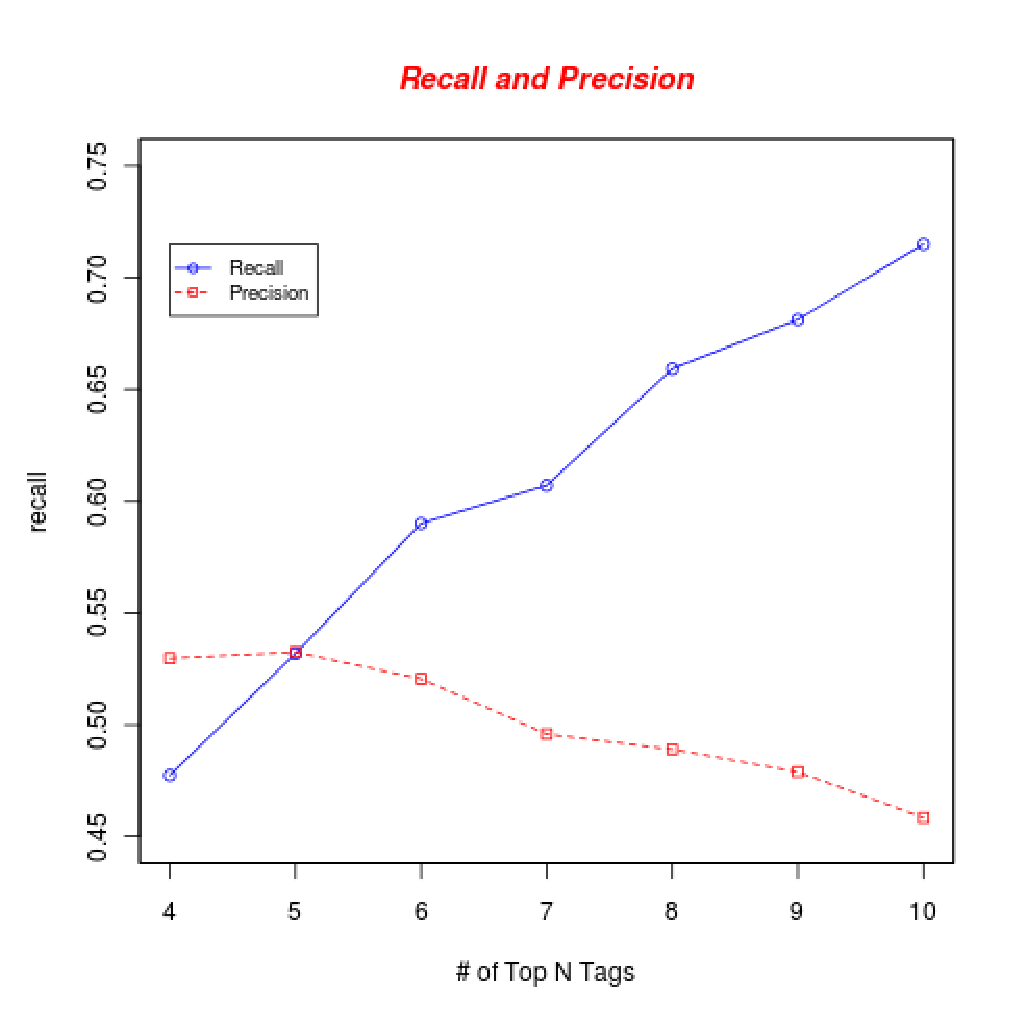
\includegraphics[scale=0.42]{naives.eps}
\caption{Tag Prediction By Naive Bayes}
\label{fig:naive}
\end{figure}

\subsubsection{Logistic Regression}
Under Construction

\subsubsection{Neural Networks}
Under Construction

\subsection{Comparison and Conclusion}
Under Construction. This part depends on the experimental results of all the three models.
